\chapter{Populaire samenvatting}

Vandaag de dag is men steeds meer bezig met het delen van informatie. Omdat het belangrijk is dat deze informatie ergens opgeslagen wordt, zijn we altijd op zoek naar \emph{compressie}: het `inpakken' van informatie zodat het minder ruimte in beslag neemt.

Bij deze compressie zijn twee types te onderscheiden. Bijvoorbeeld tekst moet na de compressie perfect ge\emph{reconstrueerd} kunnen worden. Deze tekst is een signaal wat wij niet zullen behandelen. Wij zijn ge\"interesseerd in \emph{lossy} compressie, wat betekent dat we `oninteressante informatie' gewoon weg kunnen gooien met de hoop dat de reconstructie goed genoeg lijkt op het origineel.

In het bijzonder zullen wij ons vizier richten op beeldmateriaal, eerst stil en daarna bewegend. Foto's worden veelal opgeslagen in het zogenaamde JPEG-beeldformaat: \texttt{.jpg}. De wiskunde achter dit compressie-algoritme is niet triviaal en wij zullen hier dan ook grondig op ingaan in ons verslag. De Fouriertransformatie wordt in \emph{signaalverwerking} al honderden jaren toegepast om signalen (functies, geluid, foto's, films) te schrijven in een andere \emph{basis}, namelijk de basis van de complexe $e$-machten $e^{2 \pi i t}$. We hopen hierbij maar dat ons signaal goed te benaderen valt in deze basis.

Het lot wil is dat dit helemaal niet altijd goed werkt. Mede door dit nadeel is in de laatste dertig jaar een nieuwe speler op het gebied van signaalverwerking opgedoken en dat is de zogenaamde Wavelettransformatie. In de praktijk worden deze wavelets gebruikt in een nieuwere variant van JPEG: JPEG-2000. Een wavelet is niks anders dan een functie $\psi: \R \to \R$ waarvoor geldt $\int_{-\infty}^\infty \psi(t) dt = 0$. Dit op zich is nog niet handig, maar er zijn wavelets met een zogenaamde \emph{compacte drager}. Merk op dat voor de complexe $e$-machten geldt dat de drager $\mathbb{F} = \overline{\{ t \in \R: e^{2 \pi i t} \not= 0 \}}$ gelijk is aan $\R$. Een wavelet heeft een compacte drager wanneer deze drager een compacte verzameling in $\R$ is. Zie figuur \ref{fig:samenv}.

\begin{figure}[h]
  \centering
  \begin{subfigure}{0.48\linewidth}
    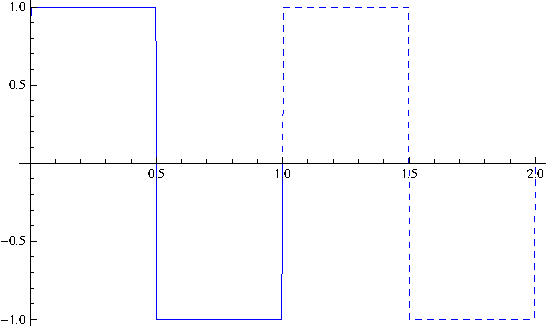
\includegraphics[width=\linewidth]{plaatjes/db1.pdf}
  \end{subfigure}
  \begin{subfigure}{0.48\linewidth}
    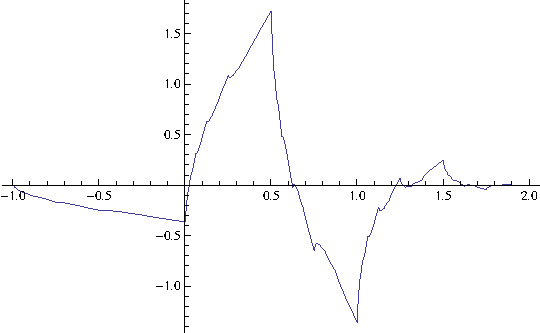
\includegraphics[width=\linewidth]{plaatjes/db2_psi.pdf}
  \end{subfigure}
  \caption{Links: De Haarwavelet. Rechts: De Daubechies-2 wavelet.}
\label{fig:samenv}
\end{figure}

Een zogenaamde orthogonale waveletbasis is nu een verzameling $\{ \psi_{j,n}: j \in \N_0, n \in \Z \}$ waarbij $\psi_{j,n}(t) = 2^{j/2} \psi(2^jt - n)$: een verschuiving over $n$ en een dilatie met factor $2^j$. Zij heet dan orthogonaal omdat de extra eis is dat zij een orthonormale basis opspant: \[\langle \psi_{a,b}, \psi_{c,d} \rangle = \delta_{a,c} \cdot \delta_{b,d}.\]

Zie wederom figuur \ref{fig:samenv} voor een grafiek van $\psi_{0,0} = \psi$ en $\psi_{0,-1}$ voor twee wavelets. De Haarwavelet is de oudste (en meest simpele) wavelet in gebruik en staat centraal in ons verslag. Rechts is de Daubechies-2 wavelet te zien. Deze hebben we als tweede wavelet ook bekeken.

De Fouriertransformatie en Wavelettransformatie geven ons op deze manier een wiskundig onderbouwde manier om signalen in \'e\'en dimensie (bijvoorbeeld geluid) te comprimeren naar een fractie van haar oorsponkelijke grootte. We hopen dan dat de reconstructie nog dichtbij het origineel lag (en het geluid goed te verstaan is). In twee dimensies gebruiken we voor de Fouriertransformatie het zogenaamde \emph{Tensorproduct} $f \otimes g$. Dit is een natuurlijke manier om meer ruimtes (in ons geval van functies) loodrecht op elkaar te zetten tot een $n$-dimensionale ruimte. In twee dimensies krijgen de basiselementen zo een tweedimensionale vorm: $(f \otimes g)(x,y) = f(x)g(y)$, waarbij $f$ en $g$ (mogelijk verschillende) basiselementen uit de eendimensionale basis zijn.

Bij de Fouriertransformatie blijkt zo'n voortzetting naar meer dimensies met het Tensorproduct gewoon goed te gaan. Bij de Wavelettransformatie zijn er twee mogelijkheden die beide gebruikt worden in de praktijk. Om dit in te zien kijken we weer naar een basisfunctie $\psi_{j,n}$. De verschuiving wordt nu aangegeven door $n$ en is niet zo interessant. Het \emph{niveau} echter wordt door $j$ gegeven en hiermee vinden we het verschil. Bij de zogenaamde Mallatdecompositie wordt nu een eis opgelegd. Wanneer we een meerdimensionaal basiselement $\psi^{(n)}$ bekijken moet het niveau van elke eendimensionale factor gelijk zijn. De drager van dit basiselement wordt op deze manier een vierkantje. Wanneer we deze eis niet opleggen komen we tot het `normale' Tensorproduct.

In het praktische deel van ons verslag hebben we beide decomposities bekeken met interessante resultaten. Het blijkt namelijk dat voor signalen met `redelijk weinig' grote sprongen het Tensorproduct een goede reconstructie geeft. Dit feit hebben we ge\"exploiteerd door een mengvorm van de Mallatdecompositie en het Tensorproduct te gebruiken in de analyse van 3D-signalen. Ook dit gaf interessante resultaten.

TODO: plaatje Mallat-decomp OF voorbeelden van compressie? ik hbe het idee dat er nog wat mist ofzo